\documentclass[10pt,twocolumn,letterpaper]{article}
\def\code#1{\texttt{#1}}
\usepackage{natbib}
%% Language and font encodings
\usepackage[french]{babel}
\usepackage[utf8x]{inputenc}
\usepackage[T1]{fontenc}
\usepackage{float}
%% Sets page size and margins
\usepackage[a4paper,top=3cm,bottom=2cm,left=3cm,right=3cm,marginparwidth=1.75cm]{geometry}
%% More packages
\usepackage{amsmath}
\usepackage{graphicx}
\usepackage[colorinlistoftodos]{todonotes}
\usepackage[colorlinks=true, allcolors=blue]{hyperref}
\usepackage{fancyhdr}
\pagestyle{fancy}
\fancyhead[R]{Profiling BoomerAMG}

\bibliographystyle{unsrt}
%% Title
\title{
		\usefont{OT1}{bch}{b}{n}
		\normalfont \normalsize \textsc{Mines ParisTech - Ms HPC-AI} \\ [10pt]
		\huge Projet d'Algèbre Linéaire Distribuée :\\ Profiling de BoomerAMG \\
}
\selectlanguage{french}
\usepackage{authblk}
\author{Julian AURIAC \& Aymeric MILLAN}
\affil{Cours de Christophe BOVET}
\date{17 Janvier 2022}
\begin{document}

%% just to make warning go away. Adjust the value after looking into the warning
\setlength\headheight{26pt}
% \rhead{{\color{blue}\rule{1cm}{1cm}}}

\lhead{\includegraphics[width=4cm]{fig/Logo_Mines_ParisTech.svg.png}}

\maketitle

%%%%%%%%%%%%%%%%%%%%%%%%%%%%%%%%%%%%%%%%%%%%%%%%%%%%%%%%%%%%%%%%%%%%%%%%%%%%%%%%
%%%%%%%%%%%%%%%%%%%%%%%%%%%%%%%%%%%%%%%%%%%%%%%%%%%%%%%%%%%%%%%%%%%%%%%%%%%%%%%%
%% RESUME
\begin{abstract}
Voici le document regroupant nos benchmarks de
\href{https://hypre.readthedocs.io/en/latest/solvers-boomeramg.html}{BoomerAMG},
inclus dans la librairie
\href{https://hypre.readthedocs.io/en/latest/index.html}{HYPRE}.

L'objectif du projet est double : il s'agit d'abord d'appliquer les méthodes de
résolution multigrilles algébriques de BoomerAMG sur des
\href{https://sparse.tamu.edu/}{matrices de problématiques réelles} au format
\code{.mtx} (Matrix Market).
Le deuxième objectif du projet est la réalisation de deux études
d'extensibilités :
\begin{description}
    \item [\textbullet\space Forte :] Avec
\href{https://sparse.tamu.edu/Janna/Emilia_923}{un problème de taille fiche}
au format Matrix Market, nous augmentons le nombre de processus MPI/CPU.
    \item [\textbullet\space Faible :] En partant de $1$ processus MPI et
d'un problème de taille $256 \times 256$, nous doublons la taille du problème
\textbf{et} le nombre de CPU qui travaillent sur le problème.
\end{description}

Nous mesurons dans les deux cas les temps d'exécutions de la résolution d'un
système de la forme $Au = f$, avec $A$ la matrice de départ (i.e l'observation),
$f$ la solution vers laquelle on veut converger (i.e le résultat) et $u$
le système que l'on cherche a trouver.

En plus de ces outils, ce projet apporte une vision générale sur les
méthodologies de développement sur des clusters de calculs comme celui du CEMEF. 
Nous avons pu approfondir les concepts tels que la réservation des coeurs de
calcul, le partage de ressources ou encore les scripts automatisés,
ici avec \code{OAR}.
\end{abstract}

%%%%%%%%%%%%%%%%%%%%%%%%%%%%%%%%%%%%%%%%%%%%%%%%%%%%%%%%%%%%%%%%%%%%%%%%%%%%%%%%
%%%%%%%%%%%%%%%%%%%%%%%%%%%%%%%%%%%%%%%%%%%%%%%%%%%%%%%%%%%%%%%%%%%%%%%%%%%%%%%%
%% RECUPERER LE CODE
\section{Récupérer le code}
Le code est disponible sur
\href{https://github.com/Aympab/HypreBoomerAMG_Benchmark}{ce repo GitHub}.
Vous pourrez aussi trouver le code et une archive dans nos repertoires
personnels sur le CEMEF. Le code est déjà compilé sur le cluster.

Nous avons ajouté l'option \code{-file} à l'exécution qui permet de préciser
un chemin d'accès relatif vers un fichier au format .mtx. Le code fonctionne
pour des \textbf{matrices carrées} uniquement. Attention, avec les options par 
défaut (e.g \code{-gamma}, le cycle AMG utilisé, V par défaut), seulement les
matrices symétriques définies positives permettent de converger vers une
solution. Nous avons téléchargé quelques matrices de ce type dans le répertoire
\code{matrices}, à la racinne du projet.

%%%%%%%%%%%%%%%%%%%%%%%%%%%%%%%%%%%%%%%%%%%%%%%%%%%%%%%%%%%%%%%%%%%%%%%%%%%%%%%%
%%%%%%%%%%%%%%%%%%%%%%%%%%%%%%%%%%%%%%%%%%%%%%%%%%%%%%%%%%%%%%%%%%%%%%%%%%%%%%%%
%% Implémentation
\section{Logique d'implémentation}

Pour le benchmarking, nous avons utilisé un script shell qui formate les données
des logs OAR en fichiers csv.
Ensuite, à l'aide de python et surtout de la librairie \code{pandas}, nous avons
traité les données pour les visualiser ici.
Les données brutes sont disponibles dans le répertoire \code{logs/} du projet.

Pour ce qui est de la lecture de fichier \code{.mtx} et le découpage sur les
différents coeurs de calculs, nous avons utilisé la librairie
\href{https://eigen.tuxfamily.org/index.php?title=Main_Page}{Eigen}.
La difficulté était premièrement de s'approprier la librairie, notamment les
méthodes pour accéder aux données brutes (i.e. \code{raw buffers}), dans le but
de les envoyer à l'autre librairie, HYPRE. L'interfaçage entre les deux
librairies a été pour nous la difficulté de ce projet (et donc l'axe
d'amélioration).

Nous avons essayé de réutiliser au maximum le code qui était déjà développé par
le professeur, vous trouverez le code commenté dans le fichier \code{tp.cpp}


%%%%%%%%%%%%%%%%%%%%%%%%%%%%%%%%%%%%%%%%%%%%%%%%%%%%%%%%%%%%%%%%%%%%%%%%%%%%%%%%
%%%%%%%%%%%%%%%%%%%%%%%%%%%%%%%%%%%%%%%%%%%%%%%%%%%%%%%%%%%%%%%%%%%%%%%%%%%%%%%%
%% ETUDE STRONG
\section{Étude d'extensibilité forte}

Dans cette partie, nous avons utilisé la matrice
\href{https://sparse.tamu.edu/Janna/Emilia_923}{Emilia923}, qui est issue d'un
problème de géomécanique. C'est une matrice symétrique définie positive avec 
$4\times 10^6$ nnz., et $923136$ lignes et colonnes.

\begin{figure}[H]
  \centering
  \caption{Profil de Emilia923}
  \includegraphics[width=0.3\textwidth]{fig/Emilia923.png}
\end{figure}

En gardant ce même problème tout au long de l'étude, nous allons augmenter 
le nombre de processus MPI en parralèle. Nous montons jusqu'à $3 \times 28 = 84$
processus car cela correspond à $3$ noeuds de calcul du cluster CEMEF complets.
Nous avons délimité par la ligne horizontale rouge le nombre de coeurs pour un
même noeud.
Voici les résultats de ces exécutions :

\begin{figure}[H]
    \centering
    \caption{Étude d'extensibilité forte}
    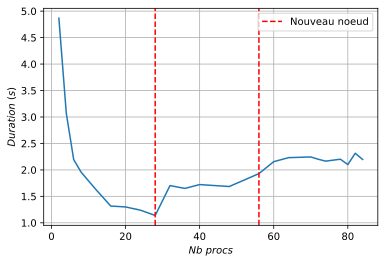
\includegraphics[width=0.45\textwidth]{fig/strong_scalab.png}
  \end{figure}

Une première chose assez flagrante que l'on peut remarquer ici est que dès que
l'on sort du même noeud de calcul, et que les communications MPI se font entre 
différents noeuds, le temps de calcul augmente.
Notons que nous avons pris soin de
réserver trois noeuds qui se trouvent côte a côte sur le cluster.

%%%%%%%%%%%%%%%%%%%%%%%%%%%%%%%%%%%%%%%%%%%%%%%%%%%%%%%%%%%%%%%%%%%%%%%%%%%%%%%%
%%%%%%%%%%%%%%%%%%%%%%%%%%%%%%%%%%%%%%%%%%%%%%%%%%%%%%%%%%%%%%%%%%%%%%%%%%%%%%%%
%% ETUDE
\section{Étude d'extensibilité faible}

Cette partie est une réalisation du sujet de TP3.

\begin{figure}[H]
    \centering
    \caption{Étude d'extensibilité faible}
    \includegraphics[width=0.45\textwidth]{fig/weak_scalab.png}
  \end{figure}


Une fois de plus, nous pouvons constater qu'il y a une divergence lorsque l'on
sort d'un seul et même noeud de calcul.

%%%%%%%%%%%%%%%%%%%%%%%%%%%%%%%%%%%%%%%%%%%%%%%%%%%%%%%%%%%%%%%%%%%%%%%%%%%%%%%%
%%%%%%%%%%%%%%%%%%%%%%%%%%%%%%%%%%%%%%%%%%%%%%%%%%%%%%%%%%%%%%%%%%%%%%%%%%%%%%%%
%% ETUDE DISTANCE
\section{Étude de l'impact de la distance physique entre deux 
noeuds sur le CEMEF}

Nous avons mis un certain temps avant de réaliser que certains de nos calculs
devenaient longs à cause de la séparation des CPUs sur plusieurs nodes. En effet
, en augmentant d'un le nombre de processus MPI, les calculs devenaient parfois
100x plus lents. En investiguant de plus près, nous nous sommes rendu compte que
non seulement être sur plusieurs nodes est coûteux en temps communication,
mais aussi que plus la distance physique entre ces noeuds de calcul est grande,
plus le temps de calcul semble multiplié.

Pour en avoir le coeur net, nous avons décidé de réaliser une dernière étude. Il
s'agit du temps de calcul pour un problème de taille fixe et pour 2 processus
MPI. L'idée est d'avoir deux CPU qui sont bien sur deux noeuds différents, et de
faire varier la distance entre ces noeuds (i.e. de choisir des noeuds plus
éloignés physiquement sur le cluster à chaque itération). Voici les résultats
que nous avons obtenus :

% \begin{figure}[H]
%     \centering
%     \caption{Étude d'extensibilité forte}
%     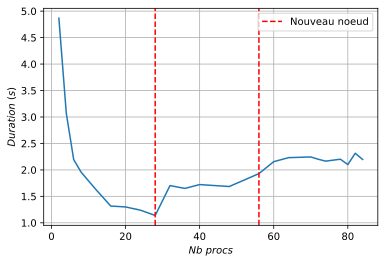
\includegraphics[width=0.50\textwidth]{fig/strong_scalab.png}
%   \end{figure}

Nous pouvons imaginer que dans un problème réel, pour couvrir le coût de ces
communications, il faudrait que le temps de calcul sur chaque processeur
soit plus important que ce temps de communication. De tout évidence, ce n'est
pas le cas pour notre problème.

\section*{Conclusions}

Les courbes que nous obtenons avec les profilings d'extensibilité forte et
faible correspondent à ce que nous avions vu en cours, il n'y a donc pas
particulièrement de surpise à ce niveau là. Cependant, l'étude "approfondie"
que nous avons mené nous a permis de découvrir de nouveaux aspects de la
programmation haute performance. Entre autres, nous avons réalisé que la
distance physique qui sépare les nodes est un facteur majeur sur la performance.
Une fois les outils et les concepts (un peu) appropriés, nous nous sommes aussi
rendus compte du confort qu'apporte l'utilisation
d'une librairie telle que HYPRE,
qui masque l'implémentation des communications MPI. C'est quand même un niveau
d'abstraction qui rend la programmation assez agréable et rassurante, tout en
nous permettant de garder un contrôle sur la performance
car nous restons dans un langage bas niveau avec le C/C++.

\section*{Axes d'amélioration}
- Split par value et pas par row car on est en CSR

- eviter le loading de la matrice pour tous les CPU pour voir la
différence entre le coup de la communication, ou alors le chargement dans 
toutes les RAM (qui est la solution naive)

- Donner la possibilité d'importer le vecteur solution depuis un fichier

- Compiler Hypre avec GPU pour faire des comparaisons (essayé sur l'ordi mais 
pas maintenu pour les nouvelles versions de CUDA, donc il faut une version de
linux datant de 2012 environ, donc c'est l'enfer pour trouver les drivers de NVIDIA
qui bougent chaque année presque)
-
\bibliography{bibliography}
\end{document}
